\chapter{Measurements from IMU}\label{IMUMeasurementsAppendix} \fxnote{find appropriate titel}
\textbf{Name: Group 630}\\
\textbf{Date: 15/04 - 2016}

\subsubsection{Purpose}
Analyse the data coming from the IMU, specifically the accelerometer and and the gyroscope measurements and calculating the angle \si{\theta_F} from those measurements.


\subsubsection{Setup}

%\begin{figure}[H]                                   
%	\centering                                        
%	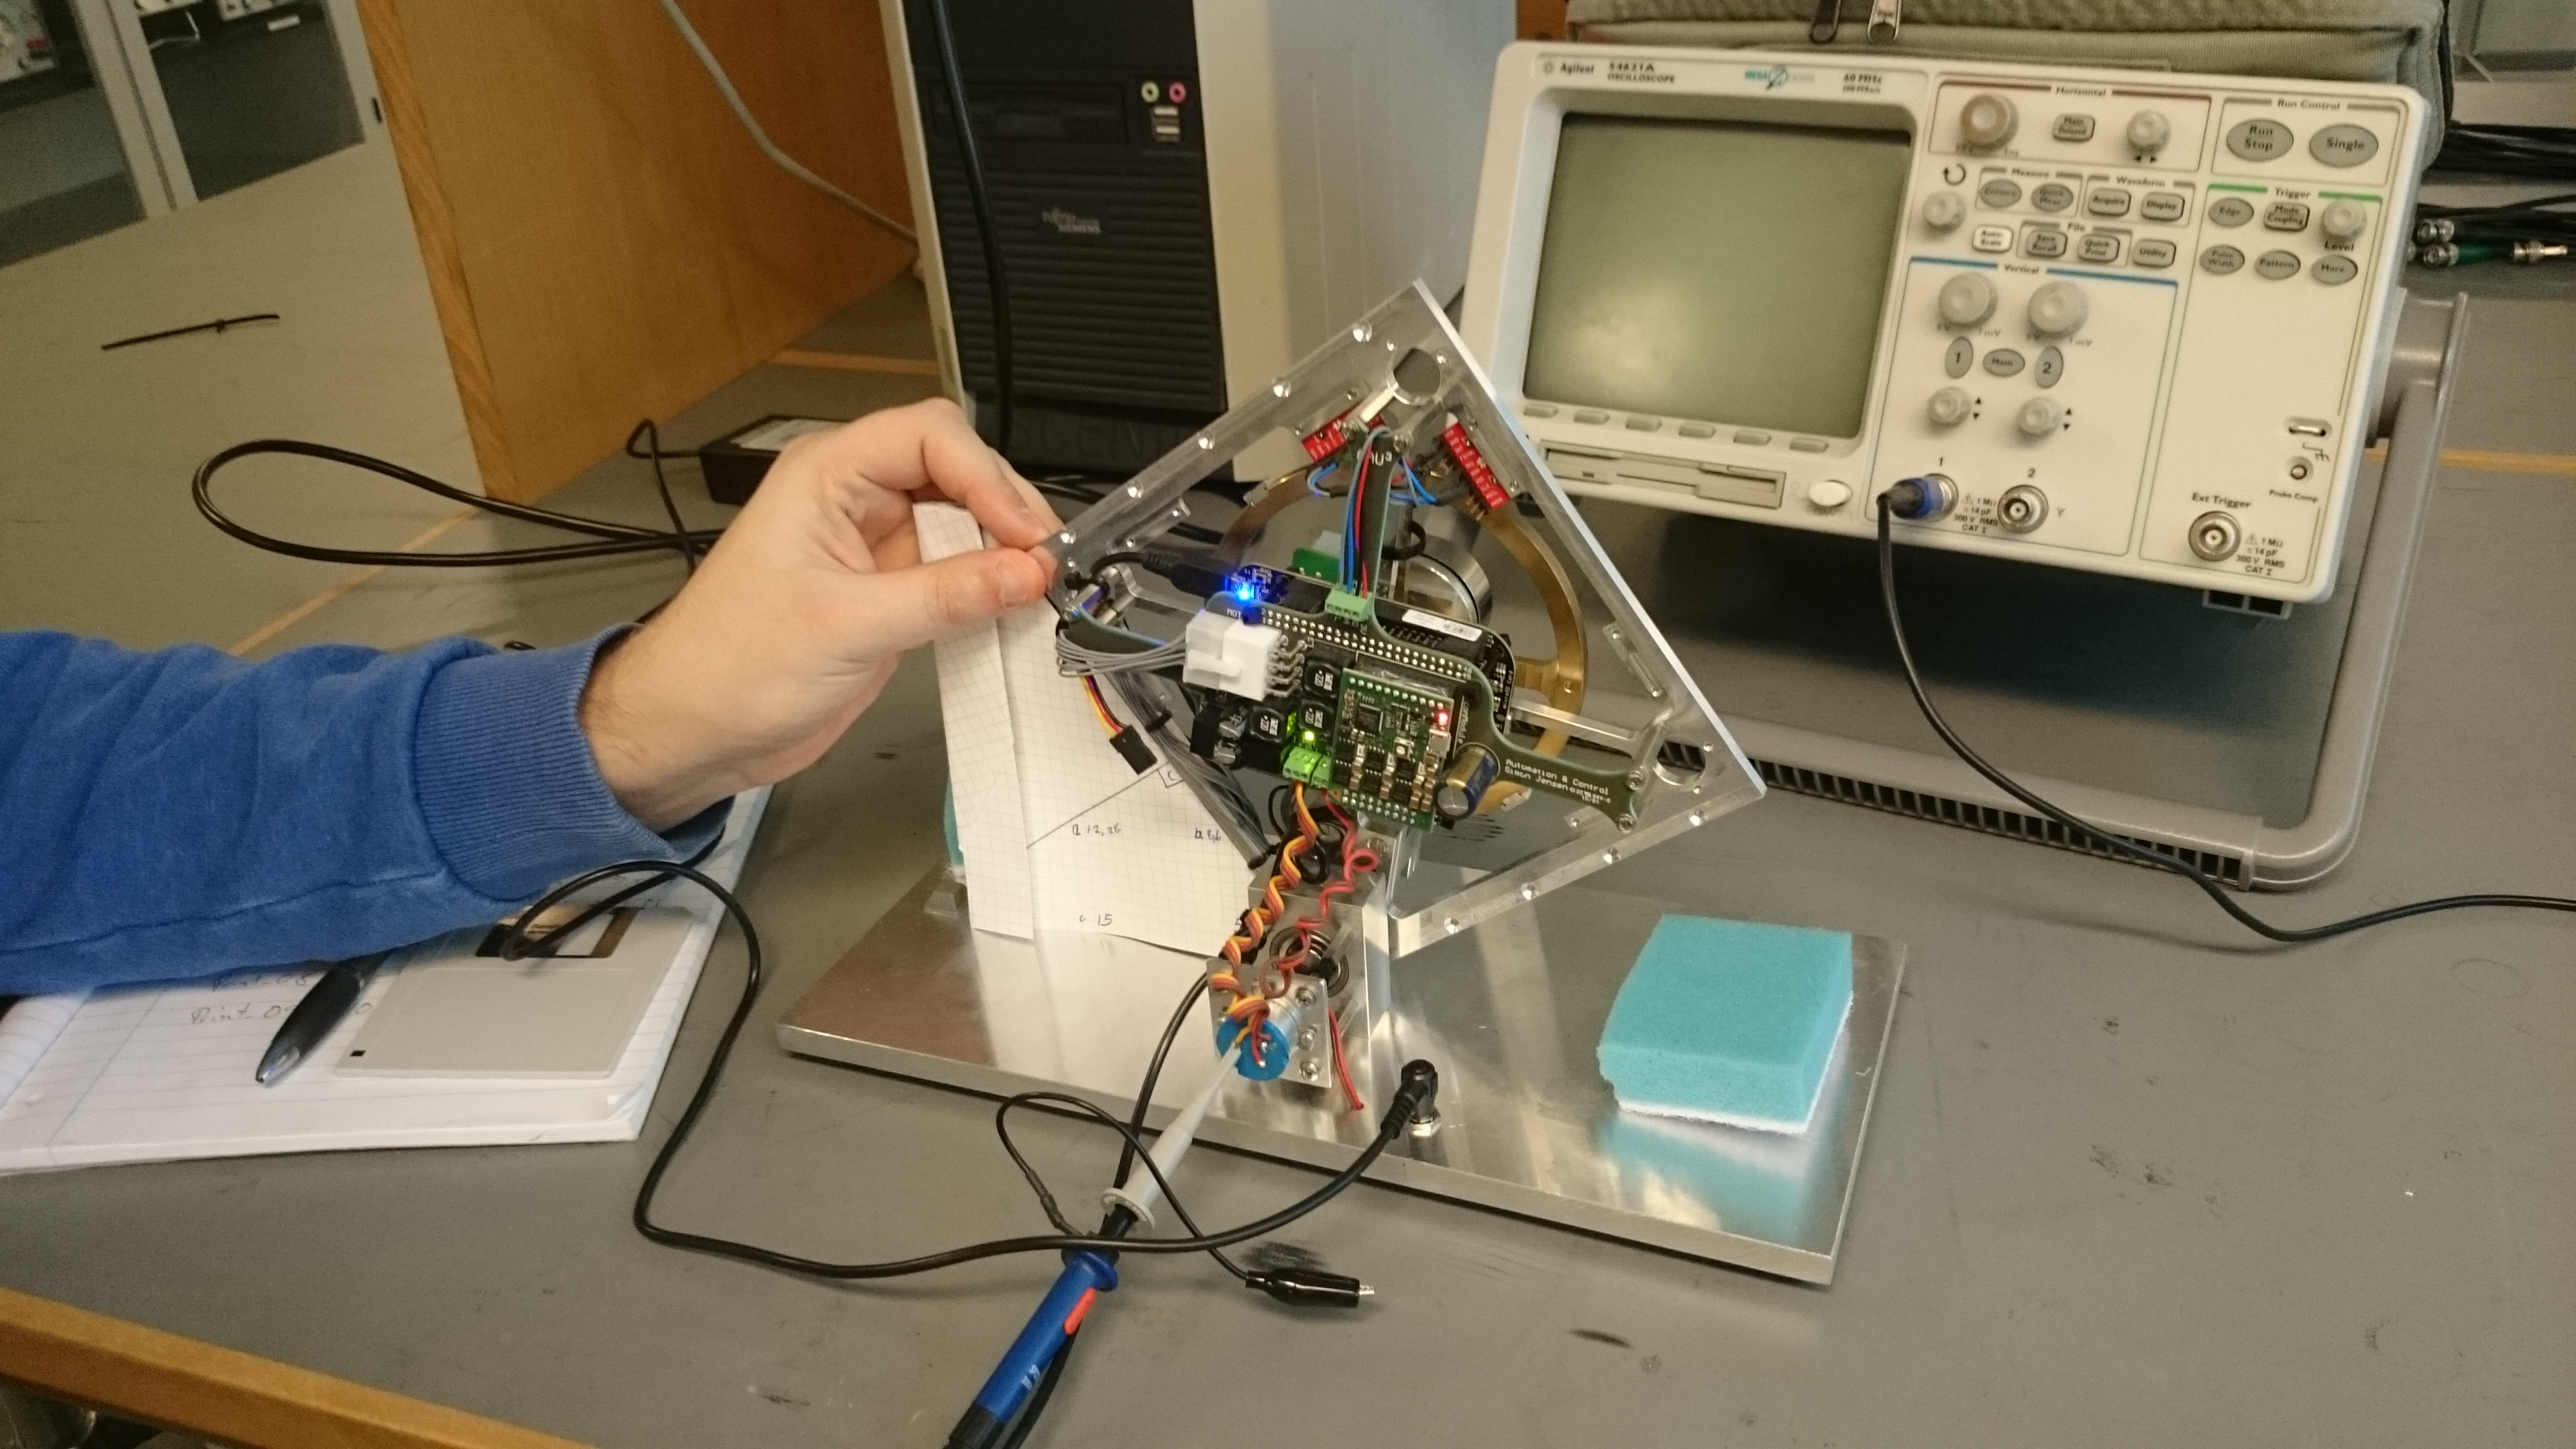
\includegraphics[scale=0.08]{figures/stepResponseSetup}
%	\caption{Picture of the data measurement test}
%	\label{dataMeasurementIMUPicture} 
%\end{figure}              

\subsubsection{List of Equipment}
\begin{table}[H]
	\begin{tabular}{|l|l|p{4.3cm}|}
		\hline%------------------------------------------------------------------------------------
		\textbf{Instrument}                        &  \textbf{AAU-no.}  &  \textbf{Type}       \\
		\hline%------------------------------------------------------------------------------------
		Cubli setup                              &               &  		  \\
		\hline%------------------------------------------------------------------------------------
		Dedicated Power Supply of Cubli \small{(24 V - 3 A)} &               &  XP Power, AEB70US24 \\
		\hline%------------------------------------------------------------------------------------
		PC with the code from simon                &              &            \\
		\hline%------------------------------------------------------------------------------------
	\end{tabular}
\end{table}
\subsubsection{Procedure}
\begin{enumerate}
	%\item Turn on the power supply
	\item Upload the code with Simons controller
	\item Start the program and let the cubli balance for a few seconds
	\item Poke the Cubli a few times so there is some random variations in the angle
	\item Take the measurements and plot them in Matlab
	%\item Plot the result of the simulations in the same figure and compare them
\end{enumerate}


\subsubsection{Results}
The measured data is partially converted through the code. Accelerometer values and gyro values are thus already in rad/s. \fxnote{might need changing if we have to redo the conversion, B}
The data is available as a .csv file on the CD\fxnote{Make sure this is put into the CD folder for copying}

\small\textbf{Placeholder text}

\subsubsection{Note}



